\chapter{Importer votre personnel AES depuis un modèle de fichier Excel}

Pour vous éviter un encodage manuel fastidieux, nous avons mis en place un système d'importation de données depuis un fichier Excel. Ce fichier  peut être généré depuis le Portail. 

\begin{attention}
Il est important de ne pas modifier la structure du fichier: ne renommez, ne déplacez, n'ajoutez et ne supprimez aucune colonne du modèle Excel. Le système attend en effet un format particulier pour l'importation des données.

Vérifiez-bien si toutes les données sont complètes car l'importation du fichier ne pourra se faire qu'une seule fois. 
\end{attention}

\section{Générer le fichier}
Rendez-vous dans "Mon Équipe" et sélectionnez l'équipe d'accueil extrascolaire de type 1. En haut de l'écran, cliquez sur \ovalbox{Importer des données AES1}, puis sur Télécharger le modèle Excel à compléter. 


\begin{figure}[!h]
    \centering
    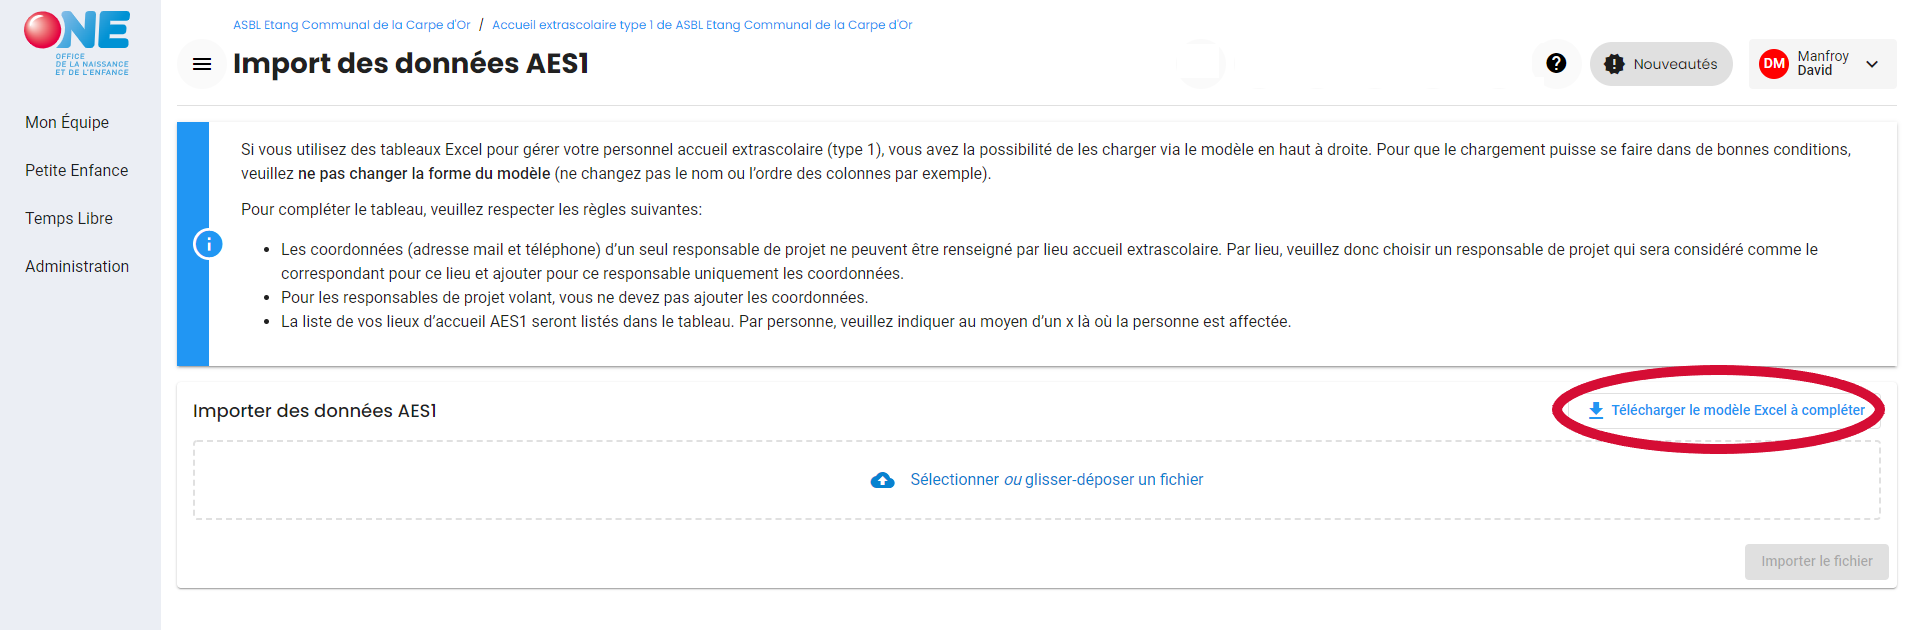
\includegraphics[width=0.8\textwidth]{Images/aes/upload_aes1/import_aes1_dl.png}
    \caption{Pour générer le fichier, cliquez sur "Télécharger le modèle Excel à compléter".}
    \label{fig:aes1_dl_modèle}
\end{figure}



\section{Compléter le fichier}
La ligne 8 du fichier vous donne le nom des colonnes. La ligne 7 vous vous fournira une explication de l'encodage attendu. Ci-dessous une explication de chaque colonne:

\subsection{Identification de la personne}
\begin{itemize}
    \item \textbf{Nom}: il s'agit du nom tel qu'il figure sur la carte d'identité de la personne. 
    \item \textbf{Prénom}: le premier prénom ou prénom usuel. 
    \item \textbf{Numéro de registre national (NRN)}: le numéro qui figure au dos de la carte d'identité belge de la personne. Si la personne est de nationalité étrangère, ne complétez pas la case. Dans ce cas, la date de naissance sera obligatoire.
    \item \textbf{NRN valide ?} : ce champ sera complété automatiquement par Excel. Il s'agit d'une formule de vérification, vous ne devez rien encoder dans cette colonne, elle se complétera automatiquement.
    \item \textbf{Date de naissance}: pour la plupart des cas, vous pourrez laisser cette colonne vide. Si la case est vide, alors le système déduira automatiquement la date de naissance sur base du NRN. 
    \item \textbf{Pays de résidence}: indiquez ici le pays de résidence de la personne.
\end{itemize}

\subsection{Relation de travail/lien contractuel}
\begin{itemize}
    \item \textbf{Relation de travail}: une liste déroulante vous affiche les valeurs disponibles: contrat, volontaires, etc.)
    \item \textbf{Date de début de contrat}: cette date est obligatoire et doit être formatée jj/mm/aaaa. 
    \item \textbf{Date de fin de contrat}: cette date est facultative.
    \item \textbf{Fraction ETP contractuel}: l'ETP de 0 à 1 de la personne dans la fonction exercée. 
    \item \textbf{Fonction ATL} : 2 choix possibles. Si la personne cumule les deux fonctions, il faut ajouter une ligne pour chacune de ses fonctions. 
        \begin{itemize}[label=\textbullet]
            \item Accueillant
            \item Responsable de projet
        \end{itemize}
    \item \textbf{Date d’entrée} dans la fonction: date à laquelle la personne a débuté dans sa fonction d'accueillant ou de responsable de projet. 
    \item \textbf{Date de sortie} de la fonction: date à laquelle la personne n'exerce plus sa fonction d'accueillant ou responsable de projet. Laisser vide si non applicable. 
    \item \textbf{Temps de travail dans la fonction}: équivalent en ETP que la personne exerce dans son rôle d'accueillant ou de responsable de projet.
    
\subsubsection{Coordonnées: uniquement pour les Responsables de projets qui sont également les personnes de contact des lieux d'accueil} 
Ces champs ne sont à remplir uniquement si le Responsable de projet est également la personne de contact du lieu d'accueil extrascolaire. 
\begin{itemize}
    \item \textbf{Adresse e-mail}: ne fournir qu'une seule adresse e-mail. 
    \item \textbf{Téléphone}: ne fournir qu'un seul numéro de téléphone. Il s'agit du numéro professionnel de la personne.
\end{itemize}
\end{itemize}

\subsection{Formation initiale}
\textbf{Formation 100 heures} (uniquement pour les accueillants extrascolaires): Renseignez ici pour les accueillants si la personne a réalisé son parcours de formation de 100h. Les deux réponses possibles sont soit oui soit non.


\textbf{Formation(s) initiale(s)}: Veuillez renseigner les diplômes reconnus de la personne (maximum deux). Une liste fermée de titres reconnus est disponible.


\subsection{Affectation par lieu d'accueil}
\textbf{Personnel volant}: le personnel volant est une personne qui n'est pas attachée à un lieu particulier, mais qui est susceptible de travailler sur les différents lieux d'accueil. Si vous mettez "oui", il ne faut pas mettre de petit x dans les colonnes des lieux.

\textbf{Personnel attaché à un (ou plusieurs) lieu(x)}: vous pouvez désigner les lieux où travaillent la personne en ajoutant un petit x dans les colonnes du lieu où preste la personne. Vous pouvez l'associer à un ou plusieurs lieux. 


\section{Importer le fichier}
Lorsque vous avez complété le fichier, vous pouvez le charger dans l'espace prévu à cet effet. Cliquez ensuite sur \ovalbox{Importer le fichier}. Le système ira chercher les données dans le fichier et ajoutera les personnes, les contrats, leur qualification (\textit{formation initiale}) et les prestations dans votre équipe d'encadrement AES1.

\begin{figure}[!h]
    \centering
    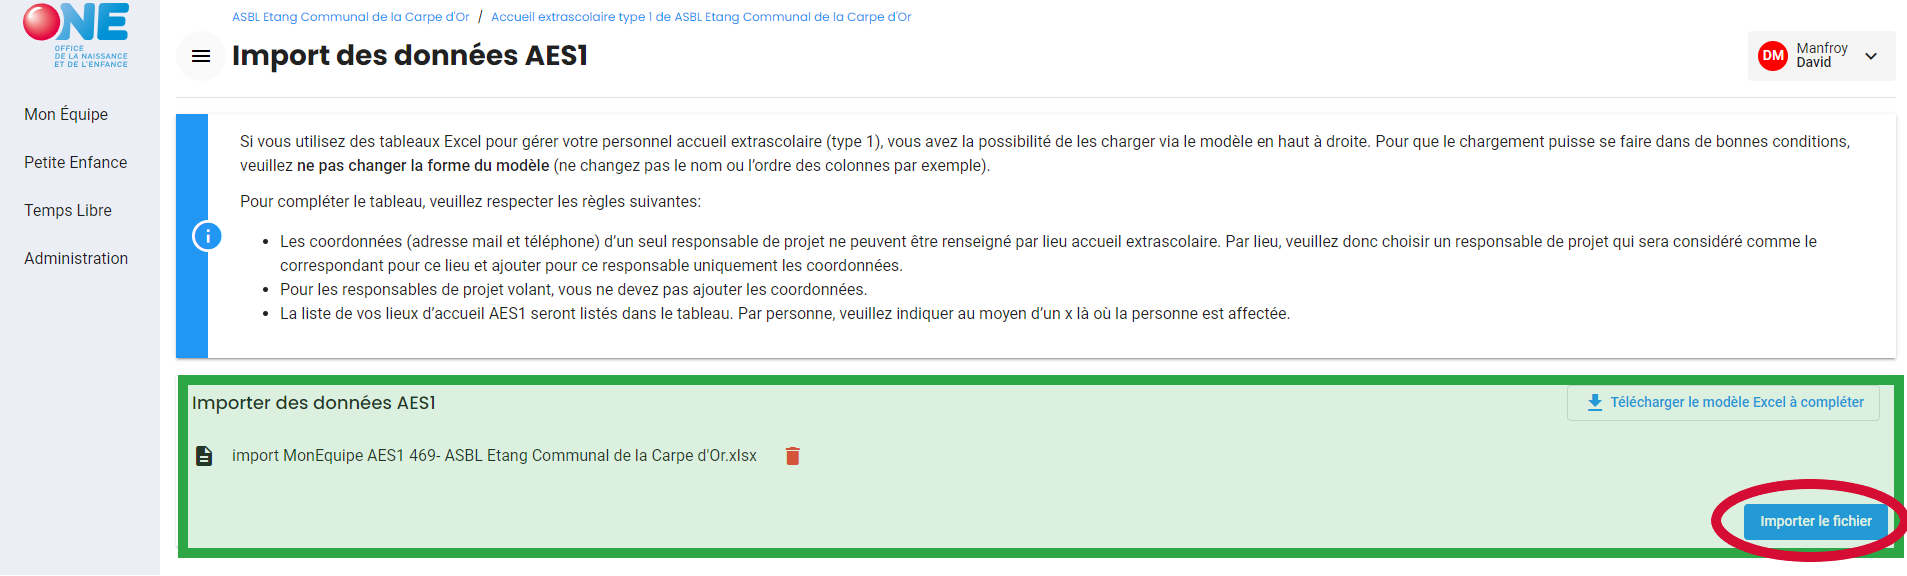
\includegraphics[width=0.8\textwidth]{Images/aes/upload_aes1/import_aes1_ok.png}
    \caption{Chargez le fichier complété en cliquant sur le petit nuage de chargement. Le système vérifie le fichier, Si le format attendu est correct, le bouton "Importer le fichier" sera disponible.}
    \label{fig:aes1_modèle_ok}
\end{figure}



\subsection{Message d'erreur}
Lorsque le fichier comporte des erreurs d'encodage, le Portail PRO vous avertira et vous indiquera dans la mesure du possible la raison. Cette indication vous aidera à corriger le fichier dans Excel.

Pour recharger le fichier corrigé, supprimez le premier fichier qui comporte des erreurs au moyen de la petite poubelle. Ensuite, chargez votre nouveau fichier.

\begin{figure}[!h]
    \centering
    \begin{subfigure}[t]{0.48\textwidth}
         \centering
         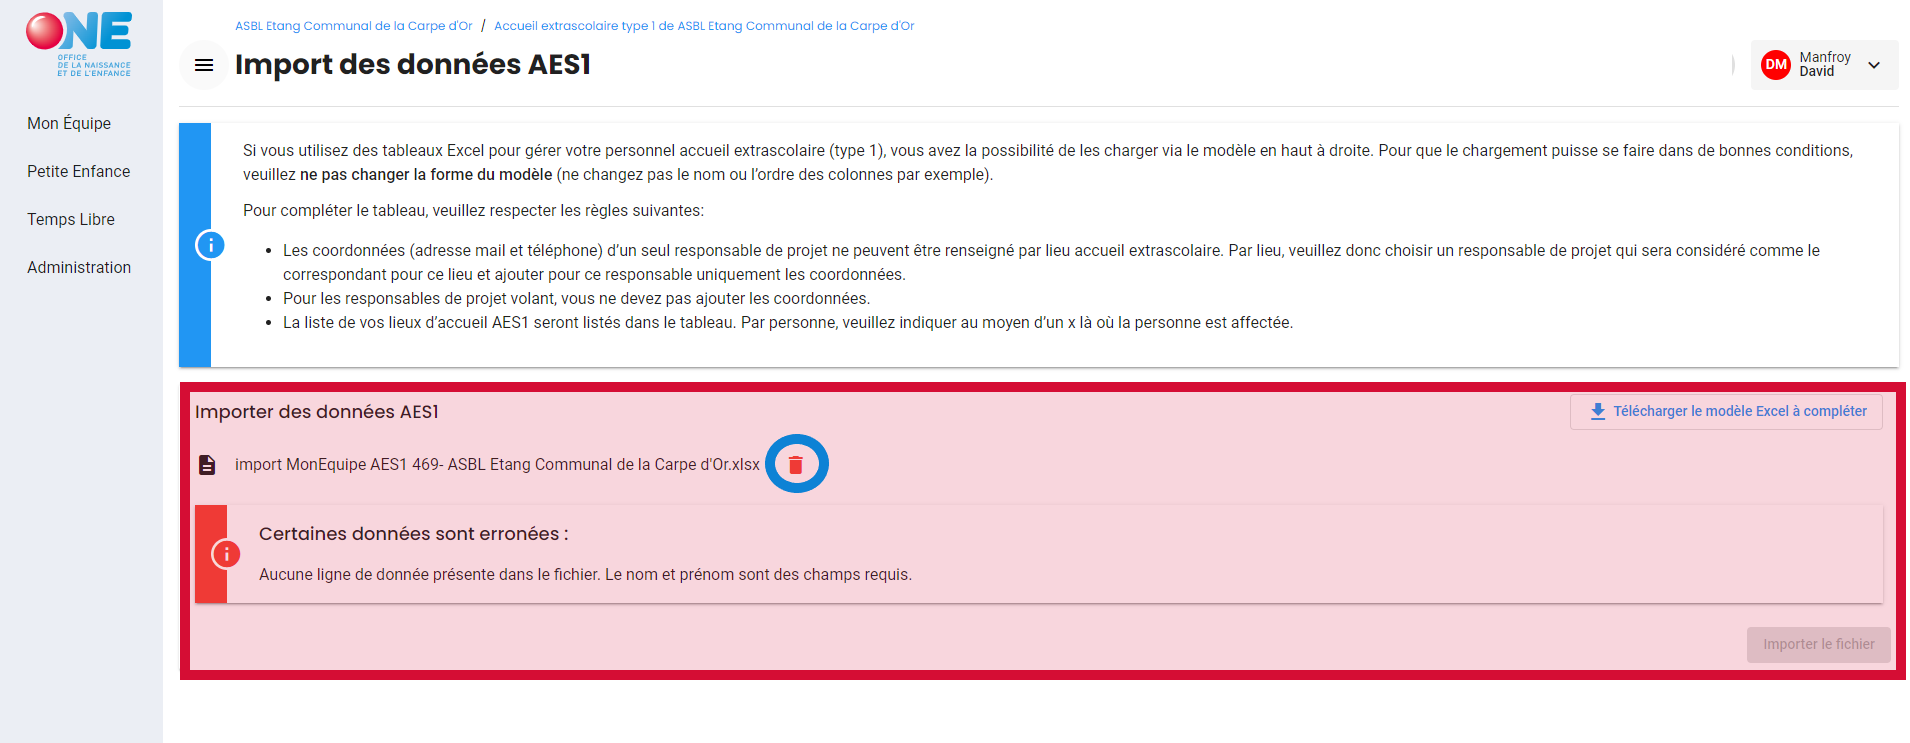
\includegraphics[width=0.95\textwidth]{Images/aes/upload_aes1/import_aes1_error.png}
         \caption{Erreur dans la structure du fichier}
         \label{subfig:modèle_erreur_structure}
     \end{subfigure}
     %\hfill
    \begin{subfigure}[t]{0.48\textwidth}
         \centering
         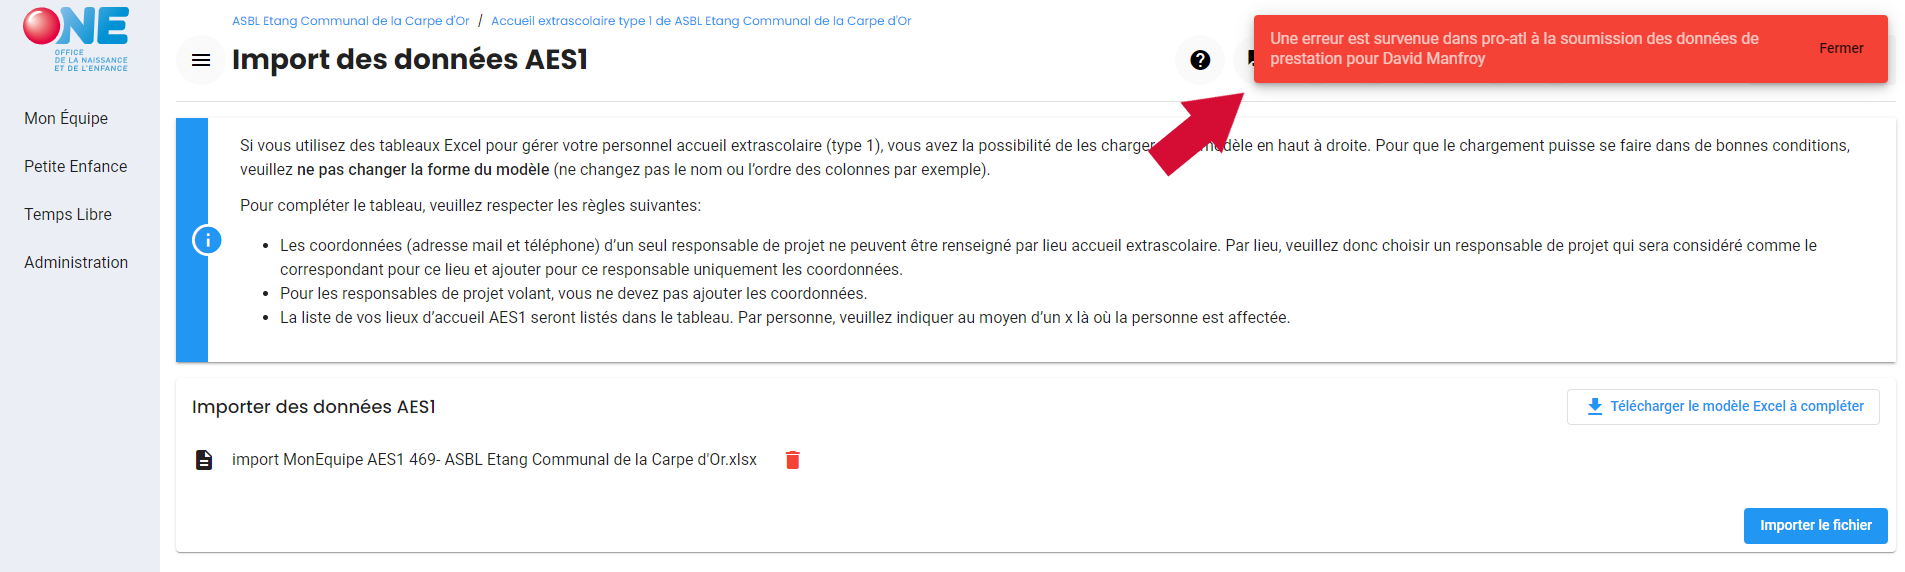
\includegraphics[width=0.95\textwidth]{Images/aes/upload_aes1/import_aes1_error_import.png}
         \caption{Erreur dans les données du fichier}
         \label{subfig:modèle_erreur_data}
     \end{subfigure}

    
    \caption{Si le fichier ne convient pas, le système vous indiquera les erreurs à corriger. Corrigez alors les erreurs, supprimez le premier fichier chargé, chargez le fichier corrigé et cliquez sur "importer les données".}
    \label{fig:aes1_modèle_erreur}
    
\end{figure}


\begin{attention}
Il n'est possible d'importer le fichier qu'une seule fois par Pouvoir organisateur ! 
\end{attention}